
% TEX TEMPLATE FILE 

% DEFINE DOCUMENT STYLE, LOAD PACKAGES
\documentclass[12pt,notitlepage]{article}		% ADD COMMENTS USING A PERCENT SIGN
\usepackage{calc}
\usepackage{amsfonts}
\usepackage{amsthm}
\usepackage{amsmath, booktabs}
\usepackage{mathtools}
\usepackage{amssymb}
\usepackage{subfig}
\usepackage[none]{hyphenat} 
\usepackage{setspace}
\usepackage{fullpage}
\usepackage{verbatim}
\usepackage{graphicx}
\usepackage{tabularx}
\usepackage{longtable}
\usepackage{multicol}
\usepackage{multirow}
%\setlength{\parindent}{0in}		% uncomment to remove indent at start of paragraphs
\usepackage{pdflscape}
\usepackage[english]{babel}
\usepackage[pdftex]{hyperref}
\usepackage{natbib}
\usepackage{caption}
\usepackage{enumitem}
\usepackage{amsmath}
\usepackage{amsfonts}
\usepackage{graphics}
\usepackage{multirow}
\usepackage{graphics}
\usepackage{hyperref}
\usepackage{longtable}
\usepackage{latexsym}
\usepackage{rotating}
\usepackage{setspace}
\usepackage{layouts} 
\usepackage[titletoc]{appendix}
\DeclareGraphicsExtensions{.pdf,.jpg,.png}
\usepackage[margin=1.25in]{geometry} % you can use the geometry package to adjust margins 
%\everymath{\displaystyle}                       % uncomment to use \displaystyle automatically in math mode


% FONTS
\usepackage[T1]{fontenc}					% always use this no matter what

% uncomment any one of these to see what it does to your font
%\usepackage{pxfonts}
%\usepackage{cmbright}
%\usepackage{txfonts}
%\usepackage[adobe-utopia]{mathdesign}
%\usepackage{kpfonts}
%\usepackage{lmodern}
%\usepackage{newtxtext,newtxmath}
\usepackage{times} 



% DEFINE WHAT GOES INTO YOUR TITLE BEFORE THE DOCUMENT BEGINS
\title{A \LaTeX\  Template}								% document title here
\author{Your Name 										% your name here
\footnote{Student, Barnard College.}}				% you can also add your institution and/or additional information in a footnote
\date{\today}											% auto-load the date

%  BEGIN DOCUMENT
\begin{document}

\maketitle			% this command typesets the title at the top of the first page

\begin{abstract}
You might want to include an abstract for your paper.  If so, you can add it here.  Your abstract will be automatically formatted and labeled.  If you do not need a formal title or an abstract, you can simply omit the code to define the title  and make the abstract and begin the document.  An abstract for this paper might include the following:  The goal of this guide is to demonstrate how to use LaTeX to produce a document.  It should help you get started but is by no means a comprehensive or exhaustive guide to LaTeX.
\end{abstract}

% If you want to have a title page, you can easily skip to the next page
 \clearpage
 
 % If you do not need a formatted title, you can also omit the steps to format and \maketitle.  Instead, you can simply add your name and any necessary information at the top of your document.
 %\noindent
 %Your Name\\
 %Course \\
 %Assignment\\
 %\date{\today}

% You can also omit the page number from your title page and start counting pages on the next page-- to do so, just un-comment the lines below (you might also want to comment out the \clearpage above)

%\thispagestyle{empty}

%\newpage

%\setcounter{page}{1}

\section{Document Sections \& Subsections}			% you can organize your doc into sections, subsections, sub-subsections, etc.

\doublespacing

Now that you have started your document, you can simply add your text.  In this section, I include several helpful commands for formatting text.  You will see bold text, italicized text, small caps, and text type text.  If you follow along in the text editor, you will notice that markup syntax, which provides formatting instructions, always starts with a backslash (\textbackslash).  In many cases, markup code also incorporates curly braces (\{ \}) to provide additional details (as with \textbackslash begin\{itemize\}) or designate text to be formatted (as with \textbackslash textbf\{bold text\}).
Here are some text formatting options:

\begin{itemize}

\item \textbf{bold text}

\item \textit{italicized text}

\item \textsc{small caps text}

\item \texttt{text type text}

\item \underline{underlined text}

\item \textbf{\textit{\underline{bold, italicized, and underlined text}}}

\end{itemize}

\subsection{Paragraphs \& Indentation}

Note that in the text editor, the sentence ``Here are some text formatting options:'' (above) appears on a new line, but when we compile the document, this sentence is continued on the previous line.\footnote{You can easily add footnotes to your document.  Here is a good place to point out how to add quotation marks in LaTeX.  You will need to type ` twice for the open quote (``) and ' twice for the close quote ('').}   If you want to skip to a new line or start a new paragraph, you will need to leave a blank line in the text editor.

The blank line tells LaTeX to start a new paragraph.  New paragraphs will automatically be indented, but you will notice that the first paragraph in each section will not be indented.  However, you may prefer to indent or not depending on a variety of considerations.  

\noindent
You can change indentation defaults if you want.  Check the next subsection-- the first paragraph is indented.


\subsection{Line Spacing}

\onehalfspacing

\indent

This document starts out double spaced, but we can easily change the line spacing.  For example, this subsection is formatted with 1.5 line spacing.  We can also use two backslashes at the end of a line followed by a blank line to skip an extra line (a single line, 1.5, or 2 lines depending on the line spacing in use).\\

Adding one or two extra lines is easy, but if we want to add more white space, we will need to use a command like ``\textbackslash vspace'' (the ``v'' is for ``vertical'') to do so.  We can also use ``\textbackslash hspace'' to add horizontal space.                As you can see, we can leave        many spaces between words in the text editor, but     when we compile the document, only one space appears between words-- unless we \hspace {10pt} add \hspace{10mm} space.


\subsection*{More on Line Spacing, Sections, \& Subsections}

\singlespacing

If you wish, you can easily use single spacing for all or part of a document.  For example, you might decide to use single spacing for subsections.  Speaking of subsections, you might have noticed that LaTeX automatically numbers your sections and subsections, but this subsection is not numbered.  If you prefer, you can omit section and/or subsection numbering by adding an asterisk (*) to the code you use to start a section or subsection.

\doublespacing

\subsection{Two Final Points about Sections and Subsections}

If you choose not to number one or more section or subsections, you can still number others.  Notice that the previous subsection is not numbered, and this subsection is 1.3 even though this is technically the 4th subsection in this section.  Finally, if sections and subsections are not appropriate or necessary for a particular document, there is no need to use them-- simply omit these commands.

\section{Typesetting Math}

You can type math in-line by sandwiching the math in between dollar signs, for example $y_i = \alpha + \beta x_i + \epsilon_i$. Underscores in math environments denote subscripting. If you want to subscript more than one character you need to put the entire subscript in curly braces like this: $X_{it}$. If you do not, it will look like this $X_it$. Similarly, superscripts (for instance when used with exponents) in math involve the use of carets like this: $x^3$ or $a^{mn}$.  You might notice that letters are automatically italicized in math environments because letters are assumed to represent variables in math mode.  If you need upright text in math mode (you might start by asking why), you can $\textup{do it}$ with the ``\textbackslash textup'' or the ``\textbackslash mathrm'' command.

If you use double dollar signs, you can center the math in its own line, for instance: $$y_i = \alpha + \beta x_i + \epsilon_i$$

You can use equation environments that allow you to align equations by whatever symbol (or lack of symbol) you place between ampersands. An example is the environment \texttt{eqnarray} where the default condition is to number equations; to remove numbering you should check the code in the .tex file below. Lines are separated by two backslashes.
\begin{eqnarray}
ATE		&=&	\textrm{E}[Y(1)] - \textrm{E}[Y(0)]	\nonumber		\\
ATE		&=& \textrm{E}[Y(1) - Y(0)]
\end{eqnarray}

Or \texttt{eqnarray*} where the default condition is to keep equations un-numbered.
\begin{eqnarray*}
ATE		&=&	\textrm{E}[Y(1)] - \textrm{E}[Y(0)]	\\
ATE		&=& \textrm{E}[Y(1) - Y(0)]
\end{eqnarray*}

Depending on your preferences and your task, you might be interested in using ``\textbackslash displaystyle,'' which can improve the appearance and readability of some mathematical expressions or equations-- particularly if you are working with fractions, integrals, or summations.  I include a few examples below.\\

Regular style:  \\

$\widehat{CACE} = \frac{\widehat{ITT}}{\widehat{ITT}_D} = \frac{\textrm{E}[Y_i(z = 1, d(1))] - \textrm{E}[Y_i(z = 0, d(0)]}{\textrm{E}[d_i(1)] - \textrm{E}[d_i(0)]} $\\

Display style:  \\

$\widehat{CACE} = \dfrac{\widehat{ITT}}{\widehat{ITT}_D} = \dfrac{\textrm{E}[Y_i(z = 1, d(1))] - \textrm{E}[Y_i(z = 0, d(0)]}{\textrm{E}[d_i(1)] -\textrm{E}[d_i(0)]} $\\\\

Regular style:\\
 
$f_1(y) = \int_{y}^{1} f(x, y) \textup{d}x$\\

Display style:\\

$f_1(y) = \displaystyle{\int_{y}^{1} f(x, y) \textrm{d}x}$\\

In the math environment, we can use the ``\textbackslash quad'' command to add space:\\

$f_1(y) = \displaystyle{\int_{y}^{1} f(x, y) \quad \textrm{d}x}$\\

Or, we can add less space by using the ``\textbackslash ;'' command:\\

$f_1(y) = \displaystyle{\int_{y}^{1} f(x, y) \, \textrm{d}x}$\\


Regular style:\\

$\textrm{E}[Y_i(1)] - \textrm{E}[Y_i(0)] = \frac{1}{N} \sum_{i=1}^N Y_i(1) - \frac{1}{N} \sum_{i=1}^N Y_i(0) $\\

Display style:\\

$\textrm{E}[Y_i(1)] - \textrm{E}[Y_i(0)] = \displaystyle{\frac{1}{N} \sum_{i=1}^N Y_i(1) - \frac{1}{N} \sum_{i=1}^N Y_i(0) }$\\

\subsection{Matrices}

LaTex also has a matrix environment for typesetting matrices.  Within the \texttt{matrix} environment, build your matrix in rows, using ampersands (\&) to separate the elements of each row into columns. \\

A basic matrix:\\

$\begin{matrix}
  a & b & c \\
  d & e & f \\
  g & h & i
 \end{matrix}$\\\\
 
 By default, elements of the matrix are centered, but you can change the alignment by adding an asterisk to the environment command  (\texttt{matrix*}) and specifying the alignment in brackets ([r], [l], [c]) after the ``\textbackslash begin\{matrix*\}'' command.  For example, you might prefer right alignment:\\
 
 
$\begin{matrix}
  -1 & 3 \\
  2 & -4
 \end{matrix} $
 \quad
 =
 \quad
 $\begin{matrix*}[r]  %% the * and the [r] create a matrix with right-aligned columns
  -1 & 3 \\
  2 & -4
 \end{matrix*}$\\\\
 
 Matrices are often enclosed in delimiters, so LaTeX allows you to incorporate delimiters into the matrix environment.  For example, \texttt{pmatrix} produces matrices enclosed in parentheses.  The example below also includes other features, such as subscripts and ellipses, that you might need to add to a matrix:\\
 
 
$A_{m,n} = 
 \begin{pmatrix}
  a_{1,1} & a_{1,2} & \cdots & a_{1,n} \\
  a_{2,1} & a_{2,2} & \cdots & a_{2,n} \\
  \vdots  & \vdots  & \ddots & \vdots  \\
  a_{m,1} & a_{m,2} & \cdots & a_{m,n} 
 \end{pmatrix}$\\\\

 

 
 Depending on your preferences or the application, you might want a different delimiter, so there are several options.   Note that you can also add an asterisk (*) to any of these matrix environments to change the column alignment.  \texttt{bmatrix} adds brackets, \texttt{Bmatrix} adds curly braces,  \texttt{vmatrix} adds vertical lines, and  \texttt{Vmatrix} adds two vertical lines:\\
  
 
$M_b = 
\begin{bmatrix}
  a & b & c \\
  d & e & f \\
  g & h & i
 \end{bmatrix}
 \quad
M_B = 
\begin{Bmatrix}
  a & b & c \\
  d & e & f \\
  g & h & i
 \end{Bmatrix}
 \quad
 M_v = 
\begin{vmatrix}
  a & b & c \\
  d & e & f \\
  g & h & i
 \end{vmatrix}
 \quad
 M_V = 
\begin{Vmatrix}
  a & b & c \\
  d & e & f \\
  g & h & i
 \end{Vmatrix}$  \\\\
 
 
 An alternative way to add delimiters is to use the ``\textbackslash right'' and ``\textbackslash left'' commands along with the delimiter you want to add.  For brackets, use the command ``\textbackslash left ['' before your matrix and ``\textbackslash right ]'' after the matrix.  Note that ``\textbackslash right'' and ``\textbackslash left'' commands can be used for other applications in addition to matrices:\\
 
 $M_b = 
 \left [
\begin{matrix}
  a & b & c \\
  d & e & f \\
  g & h & i
 \end{matrix}
 \right ]$\\
 
 If you need to index your matrix, you can use the ``\textbackslash bordermatrix'' command (note this is not a matrix environment):\\
 
 
$ M = \bordermatrix{~ & x & y \cr
                  A & 1 & 0 \cr
                  B & 0 & 1 \cr}$\\
                  
                  

\section{Tables and Figures}

Let's insert a table.  You will need to use the \texttt{table} environment and set up the basic formatting for your table.  Your code may include some details about where to place your table (in LaTeX terms, tables and figures are floats), but LaTeX will determine the exact placement of your floats.  Sometimes it can be a little tricky to deal with the placement of floats-- one option is to include [h!] in your table code (means to place the float as close as possible to where it is in your .tex file).

\begin{table}[h!]  %  [ ] the code in brackets tells LaTeX where to put the table in the text
\begin{center}  
\caption{Average Treatment Effect on Three Outcome Variables}  %  Table caption goes here (or after the table). The table number is automated
\caption*{An asterisk will print the title without numbering the table.}
\begin{tabular}{l|ccc}  %  { } the code in curly braces indicates the number of columns, alignment, and vertical lines
  \hline
  					&	Outcome Variable 1	&	Outcome Variable 2	&	 Outcome Variable 3		\\
  \hline
  Estimated ATE		& 	0.5					& 	1.2					& 	4.3			\\
  ($p$-value)			&	(0.3)				&	(0.7)				&	(0.001)		\\
  \hline
  \multicolumn{3}{l} {Note:  You can also span multiple columns.}\\
    \multicolumn{4}{r} {Note:  You can also span multiple columns and align the text on the right.}\\
\end{tabular}
\end{center}
\end{table}

 
 \subsection{Figures}

LaTeX also allows you to include figures of all kinds, including plots or graphs, maps, and pictures.  You can include figures made using a variety of applications-- basically, if you can save a figure in .pdf, .png, or .jpg format you can definitely add it to your document.  Other types of files also work (you can ask the Internet if you need help).  You might want to stick with .pdf files when you have a choice because they are less likely to pixelate if you need to adjust the size.  If the the file containing your figure is in the same folder as your LaTeX document, you can simply use the ``\textbackslash includegraphics'' command.

The example below displays a data plot from a statistical application.  You can adjust the size of the figure by specifying the width.



  \begin{figure}[!h]
\centering
\caption{A Plot}

 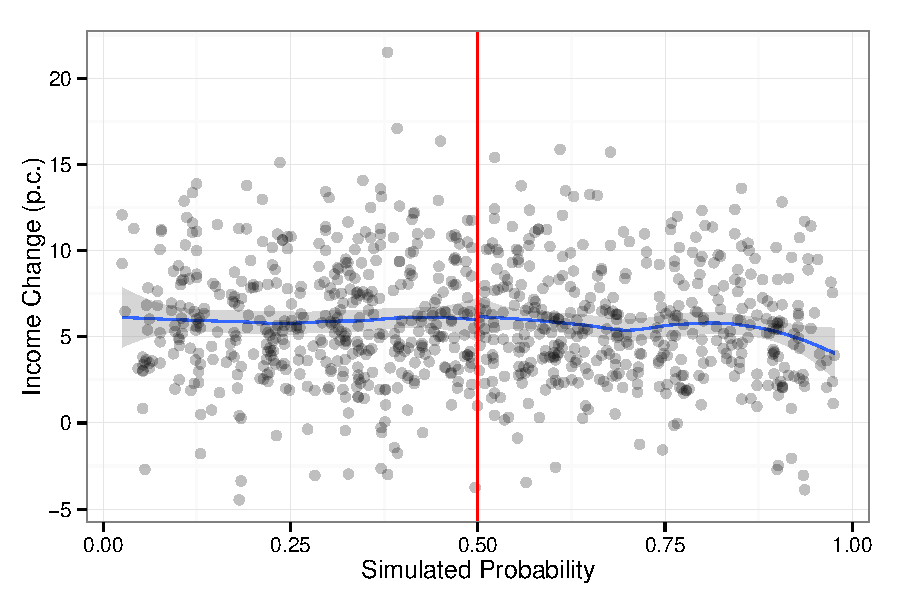
\includegraphics[width=.6\textwidth]{figure_example.pdf}  	% note the width command lets you adjust the size of the figure
 
\end{figure}


\section{Conclusion}


You can use LaTeX to produce all kinds of documents, including papers, problem sets, and presentation slides.  A lot of people use LaTeX, so if you have questions, you can usually find answers on the Internet.  It takes a while to learn the syntax and to get used to composing documents in a text editor, but it is totally worth it once you get the hang of it.  Good luck!



\end{document}



